%%%%%%%%%%%%%%%%%%%%%%%%%%%%%%%%%%%%%%%%%%%%%%%%%%%%%%%%%%%%%%%%%%%%%%
% How to use writeLaTeX: 
%
% You edit the source code here on the left, and the preview on the
% right shows you the result within a few seconds.
%
% Bookmark this page and share the URL with your co-authors. They can
% edit at the same time!
%
% You can upload figures, bibliographies, custom classes and
% styles using the files menu.
%
%%%%%%%%%%%%%%%%%%%%%%%%%%%%%%%%%%%%%%%%%%%%%%%%%%%%%%%%%%%%%%%%%%%%%%

\documentclass[12pt]{article}

\usepackage{sbc-template}

\usepackage{graphicx,url}

%\usepackage[brazil]{babel}   
\usepackage[utf8]{inputenc}  

     
\sloppy

\title{Native Language Classification\\ with Minimal Resources}

\author{Luciana P. Nedel\inst{1}, Rafael H. Bordini\inst{2}, Flávio Rech
  Wagner\inst{1}, Jomi F. Hübner\inst{3} }


\address{Instituto de Informática -- Universidade Federal do Rio Grande do Sul
  (UFRGS)\\
  Caixa Postal 15.064 -- 91.501-970 -- Porto Alegre -- RS -- Brazil
\nextinstitute
  Department of Computer Science -- University of Durham\\
  Durham, U.K.
\nextinstitute
  Departamento de Sistemas e Computação\\
  Universidade Regional de Blumenal (FURB) -- Blumenau, SC -- Brazil
  \email{\{nedel,flavio\}@inf.ufrgs.br, R.Bordini@durham.ac.uk,
  jomi@inf.furb.br}
}

\begin{document}

\maketitle

\begin{abstract}
  This meta-paper describes the style to be used in articles and short papers
  for SBC conferences.
  For papers in English, you should add just an abstract
  while for the papers in Portuguese, we also ask for an abstract in
  Portuguese (``resumo'').
  In both cases, abstracts should not have more than
  10 lines and must be in the first page of the paper.
\end{abstract}


\section{Introduction}\label{sec:introduction}

According to the International Labour Organisation (ILO) 169 agreement over native people;
it is possible to identify a group of indigenous using some aspects.
The considered features are the territory, identity recognition, common origin, culture and language \cite{povos_indigenas}.
Furthermore, according with \cite{povos_indigenas} there are 45 million native people only in Latin American.
It shows the importance of the study of their native languages and the use of computational resources to make it accessible.

Besides, computers have taken a great part of our lives, mainly in the day to day tasks \cite{matthews2016introduction}.
As the most part of the human communication is made by natural language\cite{matthews2016introduction}.
It would be of great importance the development of a process to make the human language able to be understood by the computer \cite{matthews2016introduction}.
One example of the the use of natural language processing in our day to day is the google translator \cite{google}.


Part of the task made by the google translator is classify a given text by the language and therefore is a good example of the purpose of this paper.
To accomplish this task can be used the natural language processing.
It comes from the result of the use of artificial intelligence and linguistic\cite{10.1136/amiajnl-2011-000464}.
Besides, it seeks to fill this gap between computer and the human communication.
 In addition, it has suffered a great explosion of works focusing in several languages groups\cite{peters2002evaluation}.


Therefore, considering the great importance of the native languages and its identification for a computational system.

We use the tools of the natural language processing and information retrieval to identify and classify 26 Brazilian native languages and the Portuguese.
Our task could be possible thanks to the availability of the New Testament of Bible that after some preprocessing served as a database for our project.

\section{Brazilian Native Languages} \label{sec:firstpage}
 Although, according with \cite{povos_indigenas} there are 900 thousand native people only in Brazil.

One of the biggest difficulties in natural language processing for indigenous languages is the lack of resources.

Once the languages like the ones from Tupi have a oral tradition;
there are only a few texts available for computational analyses.

Besides, the great part of languages native of Latin American, have a poly-synthetic nature.

It means that one single word can represent a whole order, and the Tupi is one of them \cite{lemos1956tupi}.
This same issue was faced on \cite{DBLP:journals/corr/abs-1804-06024} study.

The found technique to handle this problem was divide the words in the smallest morphological component to provide a wider vocabulary diverse.
Another important issue is that poly-synthetic languages of different vocabulary may have different quantities of information.


\section{Stemming}\label{sec:stemming}

The process of stemming is to reduce a word to its canonical form \cite{Goldsmith:2000:ALS:648263.753378}.
It helps us to control a database of a large set documents in the case of a identification system\cite{Goldsmith:2000:ALS:648263.753378}.
Based on that, we build the automatic stem proposed by~\cite{Goldsmith:2000:ALS:648263}.
It considers the coherence of several possible suffixes.
The coherence is calculated considering the last seven or fewer letters of a word using the equation (1).
As proposed we removed the 300 most frequent words.
After we select a stem generated by a suffix if there are at least two stems related to it.
We also consider that any used suffixes must be associated with no more than 5 stems.
Finally replaced the words for their stems.
The number of stems for each language may vary and they are shown in the figure 2.

\begin{figure}[h!]
\centering
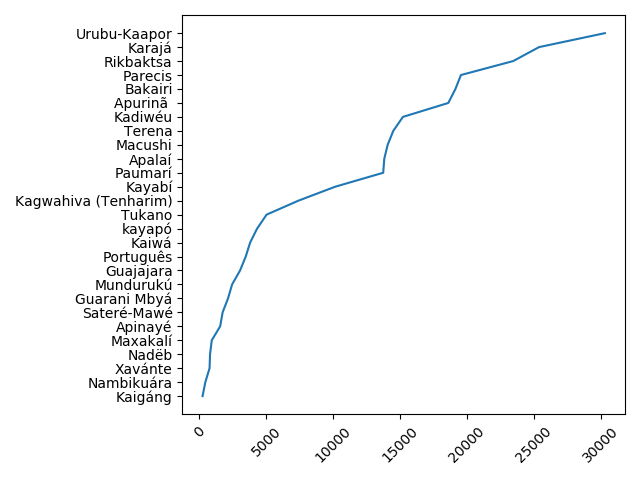
\includegraphics[width=.7\textwidth]{images/fig1.png}
\caption{Variables to be considered on the evaluation of interaction
techniques}
\label{fig:Fig1}
\end{figure}


\section{Multi-Language Classification}\label{sec:multi-language-classification}



\section{Results}\label{sec:results}

Our classification process consisted of select the 100 most frequent words of each language both in training and test set.
It was made after we use the automatic stem explained in the last section.
The training set was the first 4 books of the bible available at
\cite{angelo} and the remaining books were considered as test set.
It is important to note that a preprocessing was required before we train and test.
First we removed some HTML tags presented in the original file.
Further, we found verses that were joined in one the version of the bible, but not in the others.
Our work consisted of joined all verses where it was needed.
Finally, we check if each 100 most frequent of test was also present in the training set.
The result found is exposed in the figure 2.


\begin{figure}[h!]
\centering
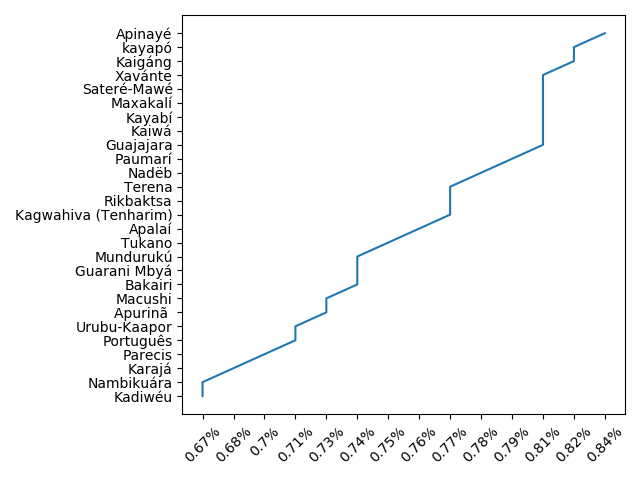
\includegraphics[width=.7\textwidth]{images/fig2.png}
\caption{Variables to be considered on the evaluation of interaction
techniques}
\label{fig:Fig2}
\end{figure}

\section{Conclusion}\label{sec:conclusion}

Considering that, even thought a world wide used translator as the google one has a lack of languages~\cite{google}.
This work tries to fill this gap introducing a method to identify Brazilian native languages.
Considering the results it is possible to affirm that even with a small text corpus it is possible to build a simple language identifier.
It was one small step in the direction of identification and classification of Brazilian languages.
Because of the simple method it can be simply added as part of a translation software as in google translator.
Furthermore, we made Brazilian native languages more accessible and ameliorate the exploration of documents writing in one of the native languages here cited.

\bibliographystyle{sbc}
\bibliography{sbc-template}

\end{document}
